\documentclass[conference]{IEEEtran}
\usepackage{cite}
\usepackage{graphicx}
\usepackage{placeins}
\usepackage{caption}
\usepackage{subfigure}
\usepackage{enumerate}
\usepackage{afterpage}
\usepackage[font={small}]{caption}
\AtBeginDocument{\renewcommand{\abstractname}{Resumo}}
\begin{document}
\title{Projeto 1 de Introdu\c{c}\~ao ao Processamento de Imagens \\ Quarta Parte}
\author{\IEEEauthorblockN{Gabriel Martins de Miranda}
\IEEEauthorblockA{130111350\\
Universidade de Bras\'ilia\\
Email:gabrielmirandat@hotmail.com}
}
\maketitle
\begin{abstract}
O presente experimento realiza o realce de uma imagem utilizando L\'ogica Fuzzy. O sistema recebe um valor de n\'ivel de cinza da imagem e atrav\'es das transforma\c{c}\~oes definidas pelas fun\c{c}\~oes de pertin\^encia substitui o valor recebido pelo valor sugerido pelo sistema de infer\^encia projetado. 
\end{abstract}

\section{ Introdu\c{c}\~ao} 
\label{sec:meth} 
Algumas considera\c{c}\~oes sobre  L\'ogica Fuzzy. A l\'ogica nebulosa diz respeito a import\^ancia relativa da precis\~ao, sendo uma maneira conveniente de se mapear um espa\c{c}o de entradas em um espa\c{c}o de sa\'idas. Desta forma, \'e f\'acil de entender e tolerante a dados imprecisos. Atrav\'es das regras de como o sistema nebuloso funcionar\'a, criamos o n\'ucleo da solu\c{c}\~ao e, atribu\'idos significados matem\'aticos a elas, temos o sistema de infer\^encia nebuloso. O processo de infer\^encia nebulosa \'e definido como o m\'etodo que interpreta os valores de entrada e, baseado nas regras do n\'ucleo, retorna os valores de sa\'ida.Os elementos cont\'em certo grau de pertin\^encia, podendo serem muito de um tipo e ao mesmo tempo pouco de outro tipo, n\~ao sendo restritos a apenas um tipo espec\'ifico. A fun\c{c}\~ao de pertin\^encia \'e aquela que mapeia o espa\c{c}o de entrada para o espa\c{c}o de sa\'ida e tamb\'em aquela que define como cada ponto do espa\c{c}o de entrada \'e mapeado em um grau de pertin\^encia, $\mu$, entre 0 e 1. O sistema ocorre da seguinte forma:

   \begin{enumerate}
	 \item Fuzzifica\c{c}\~ao das entradas: S\~ao atribu\'idos valores para cada entrada correspondentes aos seus graus de pertin\^encia.
  	\item Aplica\c{c}\~ao dos operadores nebulosos: Atrav\'es deles ($AND==min(A,B)$ $OR==max(A,B)$  $NOT==1-A$) \'e escolhido o melhor grau de pertin\^encia que representa a tal entrada.
  	\item Implica\c{c}\~ao: Sendo escolhido o melhor grau de pertin\^encia, \'e realizado um corte da fun\c{c}\~ao que descreve a sa\'ida correspondente.
  	\item Agrega\c{c}\~ao : A entrada \'e aplicada em todas as fun\c{c}\~oes de entrada e s\~ao agregrados todos os resultados de implica\c{c}\~ao.
  	\item Defuzzifica\c{c}\~ao: defuzzifica a sa\'ida agregada. Geralmente utiliza-se o $centroide$.

 \end{enumerate}
 
\section{Metodologia} 
\label{sec:meth} 
A l\'ogica Fuzzy foi implementada utilizando-se a Fuzzy Logic Toolbox (particularmente a  FIS Editor) proveniente do MATLAB. Para construir o sistema foram seguidos os passos a seguir:

\begin{itemize}
	\item Na Command Window, digitou-se $fuzzy$. O FIS Editor \'e mostrado na tela.
	\item O arquivo \'e salvo como $realce\_fuzzy.fis$.
	\item Em input1-$>$name digitou-se $entrada$.  Em output1-$>$name digitou-se $saida$
	\item Duplo clique em entrada. Em mf1: 
		\begin{enumerate}[(a)]
			\item Name = $escuro$
			\item Type = $trapmf$
			\item Params = $[-63.93$ $-20.33$ $92.77$ $137.1]$
		\end{enumerate}
		Em mf2: 
		\begin{enumerate}[(a)]
			\item Name = $cinza$
			\item Type = $gbellmf$
			\item Params = $[19.1$ $1.977$ $128]$
		\end{enumerate}
		Em mf3: 
		\begin{enumerate}[(a)]
			\item Name = $claro$
			\item Type = $trapmf$
			\item Params = $[122.2$ $161.2$ $322.2$ $361.2]$
		\end{enumerate}
   
	\item Duplo clique em saida. Em mf1: 
		\begin{enumerate}[(a)]
			\item Name = $maisescuro$
			\item Type = $trapmf$
			\item Params = $ [-33.8$ $-32.8$ $1.69$ $57]$
		\end{enumerate}
		Em mf2: 
		\begin{enumerate}[(a)]
			\item Name = $cinza$
			\item Type = $gaussmf$
			\item Params = $ [39.1$ $128]$
		\end{enumerate}
		Em mf3: 
		\begin{enumerate}[(a)]
			\item Name = $maisclaro$
			\item Type = $trapmf$
			\item Params = $ [197.3$ $254$ $313$ $319]$
		\end{enumerate}
	\item O Range foi  setado para  $[0 255]$.
	\item Em edit-$>$ rules. 
		\begin{enumerate}
			\item if entrada is $escuro$ Them saida is $mais escuro$.
			\item if entrada is $cinza$ Them saida is $cinza$.
			\item if entrada is $claro$ Them saida is $mais claro$.
		\end{enumerate}
	\item Ap\'os isto o arquivo foi salvo e fechado.
	\item O sistema de Logica Fuzzy foi conclu\'ido.
	\item O programa consiste em: para cada pixel da imagem lida, o sistema Fuzzy \'e chamado e a sa\'ida do sistema substitui o pixel da entrada.
	
\end{itemize}

\section{Resultados} 
\label{sec:meth} 
Resultados previstos na $Metodologia$:

		\vspace{2\baselineskip}\vspace{-\parskip}
		\begin{minipage}{\linewidth}
  		\centering
  		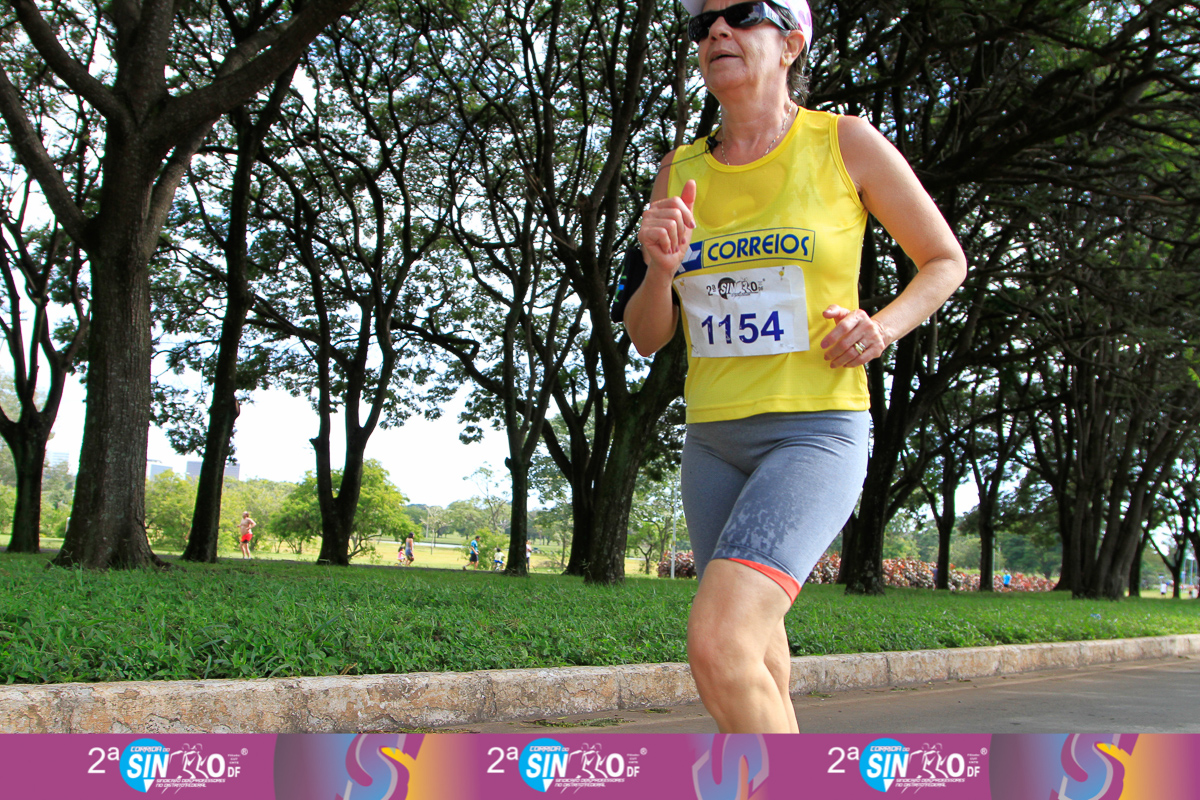
\includegraphics[width=3.3in]{../images/1}
  		\captionof{figure}{Janela do FIS Editor ap\'os o comando $fuzzy$ na Command Window.}
		\end{minipage}
		

		\begin{minipage}{\linewidth}
  		\centering
  		
\includegraphics[width=3.3in]{../images/2}
  		\captionof{figure}{Janela do FIS Editor ap\'os defini\c{c}\~ao dos nomes para input e output.}
		\end{minipage}
 		

		\begin{minipage}{\linewidth}
  		\centering
  		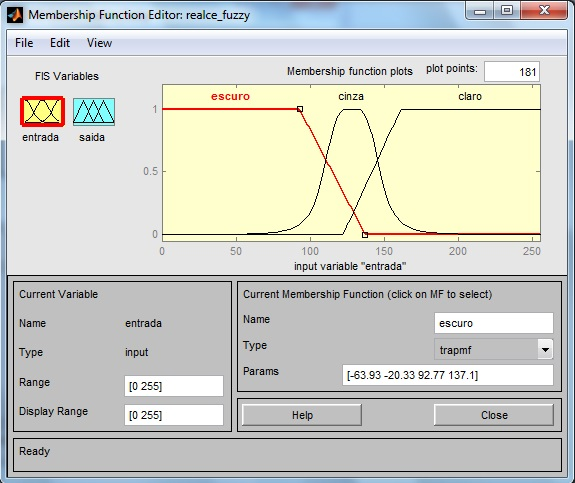
\includegraphics[width=3.3in]{../images/3}
  		\captionof{figure}{Janela do FIS Editor na defini\c{c}\~ao das fun\c{c}\~oes de entrada.}
		\end{minipage}
 		
 
		\begin{minipage}{\linewidth}
  		\centering
  		
\includegraphics[width=3.3in]{../images/4}
  		\captionof{figure}{Janela do FIS Editor na defini\c{c}\~ao das fun\c{c}\~oes de sa\'ida.}
		\end{minipage}		
 		

		\begin{minipage}{\linewidth}
  		\centering
  		
\includegraphics[width=3.3in]{../images/5}
  		\captionof{figure}{Rule Editor mostrando a defini\c{c}\~ao das regras.}
		\end{minipage}
		 		

		\begin{minipage}{\linewidth}
  		\centering
  		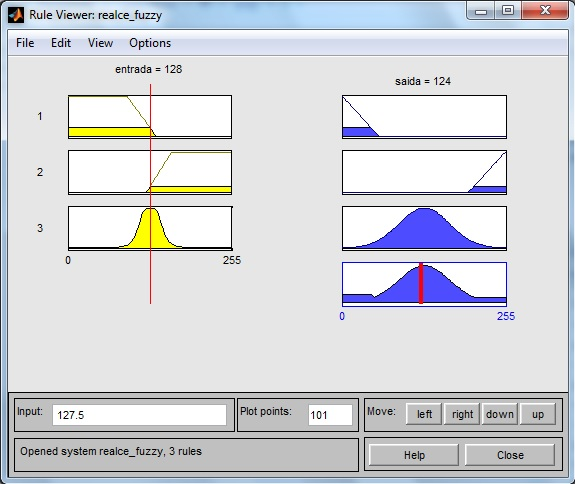
\includegraphics[width=3.3in]{../images/6}
  		\captionof{figure}{Exemplo da resposta do sistema para um valor cujo grau de pertin\^encia recai em $cinza$.}
		\end{minipage}	
	
	\vspace{2\baselineskip}\vspace{-\parskip}			
 	\vspace{2\baselineskip}\vspace{-\parskip}
           	\begin{minipage}{\linewidth}
  		\centering
  		
\includegraphics[width=3.3in]{../images/waitbar}
  		\captionof{figure}{Janela de espera para enquanto o sistema realiza todas as etapas em cada $pixel$. }
		\end{minipage}			
		

 			\vspace{2\baselineskip}\vspace{-\parskip}		 		
 			\vspace{2\baselineskip}\vspace{-\parskip}		 						 						 						 		\vspace{2\baselineskip}\vspace{-\parskip}	
		 	\vspace{2\baselineskip}\vspace{-\parskip}				 			
		 	\vspace{2\baselineskip}\vspace{-\parskip}		 									\vspace{2\baselineskip}\vspace{-\parskip}				 				 	Os resultados ocorreram como previsto. Os n\'iveis escuros ficaram ainda mais escuros, os claros ainda mais claros e os cinzas permaneceram em uma faixa aceit\'avel. Os valores extremos(muito escuro e muito claro), na faixa de n\'iveis de cinza de $[0,19.1]$ e $[236,255]$, por\'em, n\~ao apresentaram valores muito satisfat\'orios, como pode ser visto em $Fig.8$ e em $Fig.9$. 	
		 	\vspace{2\baselineskip}\vspace{-\parskip}	
		 	\vspace{2\baselineskip}\vspace{-\parskip}		 		
		\vspace{2\baselineskip}\vspace{-\parskip}
		\begin{minipage}{\linewidth}
  		\centering
  		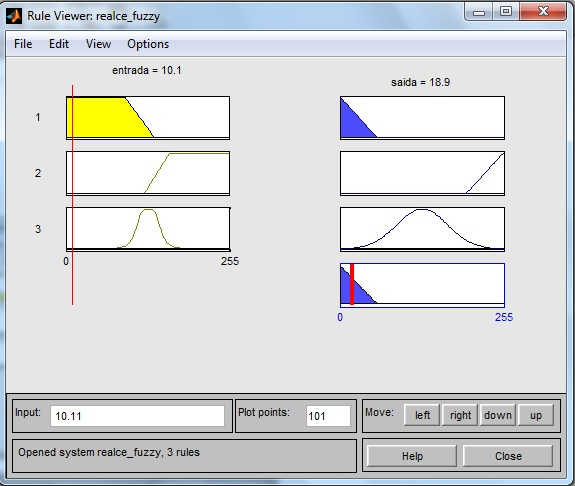
\includegraphics[width=3.3in]{../images/7}
  		\captionof{figure}{Exemplo da resposta do sistema para um valor muito escuro. O sistema n\~ao conseguiu atribuir um valor $mais$ $escuro$ para ele.}
		\end{minipage}	
	
	\vspace{2\baselineskip}\vspace{-\parskip}	
	\vspace{2\baselineskip}\vspace{-\parskip}	
		\begin{minipage}{\linewidth}
  		\centering
  		
\includegraphics[width=3.3in]{../images/8}
  		\captionof{figure}{Exemplo da resposta do sistema para um valor muito claro. O sistema n\~ao conseguiu atribuir um valor $mais$ $claro$ para ele.}
		\end{minipage}
		
		\vspace{2\baselineskip}\vspace{-\parskip}	
		\vspace{2\baselineskip}\vspace{-\parskip}	
		
		\vspace{2\baselineskip}\vspace{-\parskip}
	
S\~ao apresentadas tr\^es imagens ap\'os utiliza\c{c}\~ao do sistema fuzzy: $a$) $characters\_test\_pattern$, $b$) $Lena$ e $c$) $Baboon$.
		\vspace{2\baselineskip}\vspace{-\parskip}
		\\
		

		\begin{minipage}{\linewidth}
  		\centering
  		
\includegraphics[width=3.3in]{../images/9}
  		\captionof{figure}{Antes.}
		\end{minipage}				


		\begin{minipage}{\linewidth}
  		\centering
  		
\includegraphics[width=3.3in]{../images/10}
  		\captionof{figure}{Depois.}
		\end{minipage}	
 		
 		$a$) $characters\_test\_pattern$
 		
 		
 		
		\begin{minipage}{\linewidth}
  		\centering
  		
\includegraphics[width=3.3in]{../images/11}
  		\captionof{figure}{Antes.}
		\end{minipage}				

		\begin{minipage}{\linewidth}
  		\centering
  		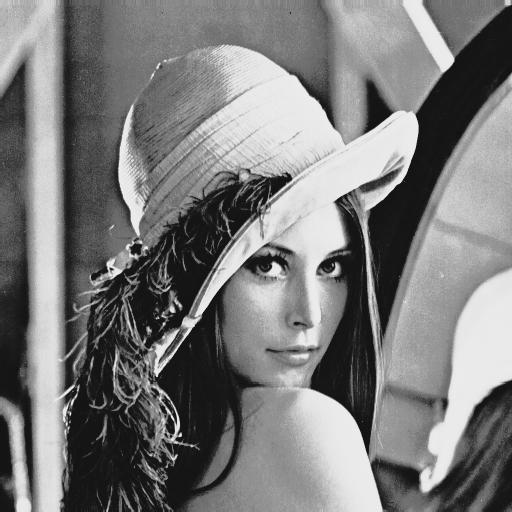
\includegraphics[width=3.3in]{../images/12}
  		\captionof{figure}{Depois.}
		\end{minipage}	

		$b$) $Lena$
		
 	
		\begin{minipage}{\linewidth}
  		\centering
  		
\includegraphics[width=3.3in]{../images/13}
  		\captionof{figure}{Antes.}
		\end{minipage}				

		\vspace{2\baselineskip}\vspace{-\parskip}
		\vspace{2\baselineskip}\vspace{-\parskip}
		\begin{minipage}{\linewidth}
  		\centering
  		
\includegraphics[width=3.3in]{../images/14}
  		\captionof{figure}{Depois.}
		\end{minipage}	
		
		\vspace{2\baselineskip}\vspace{-\parskip}
		\vspace{2\baselineskip}\vspace{-\parskip}
		\vspace{2\baselineskip}\vspace{-\parskip}			
 		$c$) $Baboon$		
	
\section{Conclus\~ao} 
\label{sec:meth} 

Foi poss\'ivel concluir os benef\'icios do uso do sistema Fuzzy para real\c{c}ar o contraste de imagens, sua facilidade de implementa\c{c}\~ao e resultados finais impressionantes, apesar dos valores extremos n\~ao se adequarem totalmente as regras  j\'a que o sistema atende ao m\'etodo de $centroide$, sendo imposs\'ivel obter uma fun\c{c}\~ao cuja centr\'oide ca\'isse no valor $zero$, no caso em que a entrada fosse $0$.

\section{Refer\^encias} 
\label{sec:meth} 

[1] R. C. Gonzalez and R. E. Woods, Digital Image Processing,
Prentice-Hall, EUA, 2nd edition, 2002.
\end{document}